\section{Performance Analysis / Evaluation}

In this section, a performance analysis is done on all algorithms implemented in walky. Where applicable, problem size scaling, strong scaling, and \ac{MPI} scaling analysis are done per algorithm. With problem size scaling, the problem size is increased with a fixed amount of parallelism while with strong scaling, the parallelism is increased with a fixed problem size. Due to the missing Score-P support for LLVM and especially cargo, the \ac{MPI} analysis was done purely mathematically.
\subsection{Cluster Setup}

The benchmarks were done on the \ac{SCC} at GWDG, the joint data center of Max Planck Society for the Advancement of Science (MPG) and University of Göttingen.\footnote{\href{https://gwdg.de/en/hpc/systems/scc/}{\url{https://gwdg.de/en/hpc/systems/scc/}}}. The \ac{SCC} is a large \ac{HPC} system, consisting of about 410 compute nodes with over 18000 CPU cores, 99TB RAM, and 5.2 PiB of storage, split into two filesystems.
For our benchmarks, the so-called \texttt{amp} node type, of which 96 exist at the \ac{SCC}, was used. An \texttt{amp} node has two Xeon Platinum 9242 with a total of 48 CPU cores running at a frequency of 3.8 GHz. Each node has 384 GB of RAM. The jobs were assigned using the internal SLURM workload manager.

\subsection{Vampir-based Analysis of Rust \acs{MPI} Code}

It was initially planned to do the distributed analysis of the \ac{MPI} code using Vampir \cite{noauthor_vampir_nodate}.
Vampir internally uses Score-P \cite{brunst_score-p_2012} for the generation of trace log files. 

Unfortunately, Score-P is not supported by the Rust compiler.
While there is literature to show that Score-P can be integrated into the \acs{LLVM} ecosystem \cite{tschuter_llvm_2017}, the source code was never released.
Furthermore, what makes matters worse is that, even if the tool were published, it is still not trivial to include it into
the cargo build process, which is required for building our third-party dependencies\footnote{As many modern languages do, 
Rust does not specify an \ac{ABI} and instead recompiles all subdependencies (for bounds, the C 
\ac{FFI} convention is usually used). This means, that one can't just link against system-wide libraries as in C.}.

Note that this problem is not just contained to Vampir. Other common analysis tools such as Scalasca \cite{noauthor_scalasca_nodate} or TAU \cite{noauthor_tau_nodate} also rely on Score-P internally.

Therefore, the \ac{MPI} analysis will be theoretically by mathematically scaling the number of messages and bytes sent as well 
as their temporal relationship.

\subsection{Exact Solving Benchmarks}

\subsubsection{Problem Size Scaling}

All single threaded iterations of the algorithm, together with the rayon-based multithreaded version with 24 threads, were run for 24h on the cluster, sequentially computing a random graph from size 3 to size 50. Here are the results:
\begin{figure}[H]
    \centering
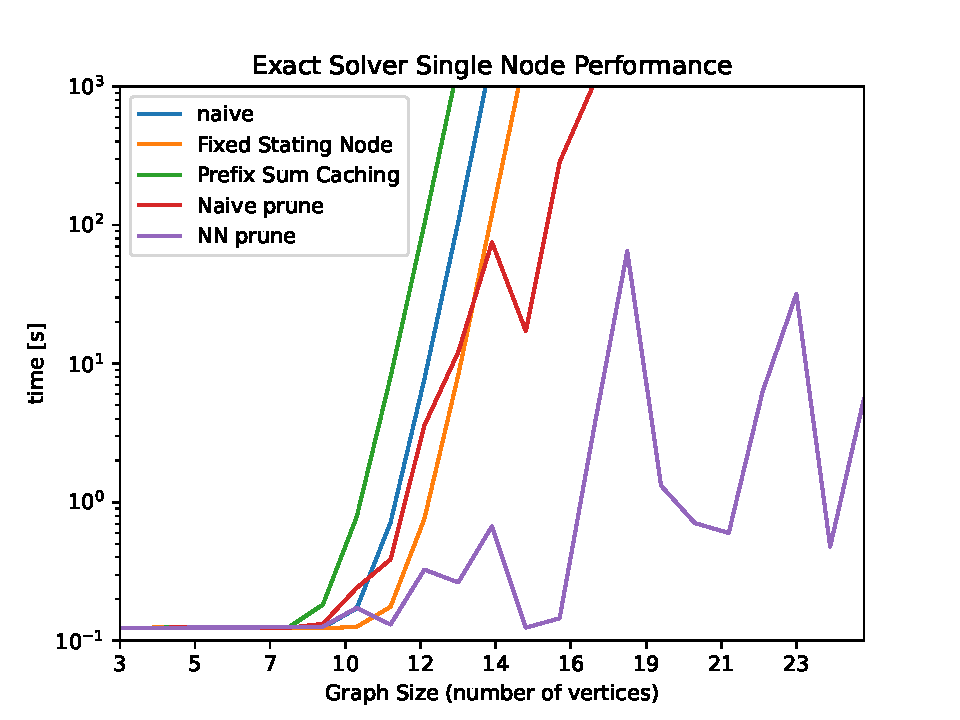
\includegraphics[width=0.8\textwidth]{./assets/exact-stmt1.pdf}
\caption{} % generates a (a)
    \caption{The results of the exact solver. shows all algorithms until the NN prune}
\end{figure}

\begin{figure}[H]
    \centering
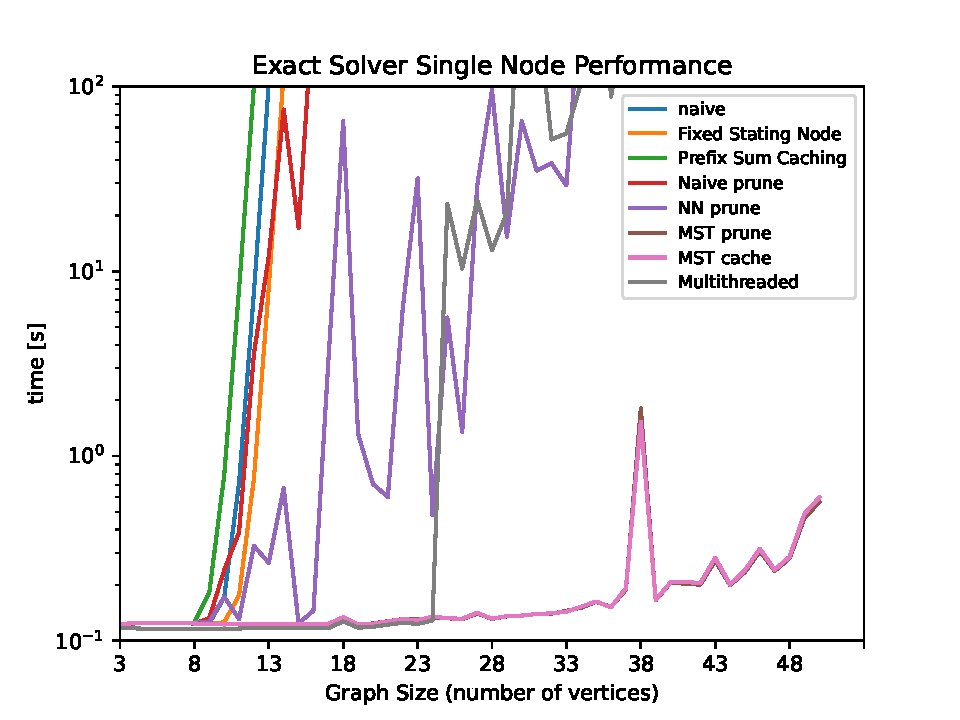
\includegraphics[width=0.8\textwidth]{./assets/exact-stmt.pdf}
\caption{} % generates a (a)
    \caption{The results of the exact solver. shows all algorithms with a smaller $y$-axis}
\end{figure}

For the full results see Table \ref{tab:exact_benchmarks} in the appendix.

The most important insight is that pruning, especially \acs{MST}-based pruning, immensely improves the viability of exact solving. While $n=14$ took over $20$ minutes with the na\"ive version, it was computed in around $0.11$ seconds using the optimized pruner. It was possible to compute $n=50$ in around $0.3$ seconds\footnote{The benchmark was stopped at $n=50$.}.

Other important insights include the following:
\begin{itemize}
    \item The prefix sum caching was even slower than the na\"ive implementation! This was because we changed from the fast iterative permutation algorithm to recursive enumeration. There are several reasons why this is such slow, from function call overhead to less compiler optimization opportunities to not being tail call optimized. But by the time na\"ive pruning was used, it already consistently outperformed the initial $v0$ on the randomly generated graphs.
    \item While pruning generally improves performance, it does not improve performance deterministically, which is shown in the spikes on less-prunable graphs.
    \item The \ac{MST} performance is insanely good. Remember that this is still an $\mathcal{O}(n!)$ worse case algorithm.
    \item The caching did not improve the previous algorithm enough to justify the added complexity. In fact, depending on the graph, it could worsen overall performance.
\end{itemize}

Last but not least, the multithreaded version performed way worse than the sequential one it was based upon. There are several possible reasons for this behaviour: \label{rayondoof}
\begin{itemize}
    \item Context-switching and threading overhead caused by the operating system.
    \item Blocking inter-thread locking on the current best solution, which was in a mutex that every thread got an atomically reference counted pointer for.
    \item Worse cache utilization. The more threads run on the system, the more context switching. Every time the thread is switched, the CPU caches are flushed by the previous program. Furthermore, hyperthreading always at least halves the cache if not destroys it completely by two threads greedily competing for it.
\end{itemize}

\subsubsection{Strong Scaling}

The strong scaling analysis of the \ac{MPI}-based, distributed exact solver requires a more sophisticated analysis. Before looking at the plotted data, let us compare the statically allocated (V0) algorithm to the dynamically allocated (V1) algorithm:

\begin{table}[H]
\centering
    \begin{tabular}{|c|c|c|c|c|c|c|c|}
        \hline
        Type & Total Worker & V0 $\mu$ & V0 $\sigma$ & V0 Efficiency & V1 $\mu$ & V1 $\sigma$ & V1 Efficiency\\
        \hline
        1n2p & 2 & 815.612 & 0.485 & 72.093 & 134.508 & 0.062 & 437.148\\
        2n1p & 2 & 815.850 & 0.453 & 72.072 & 134.787 & 0.091 & 436.245\\
        1n4p & 4 & 750.874 & 1.011 & 39.154 & 100.460 & 9.940 & 292.654\\
        4n1p & 4 & 746.932 & 0.678 & 39.361 & 63.301 & 0.077 & 464.451\\
        8n1p & 8 & 19.223 & 0.075 & 764.690 & 38.952 & 0.069 & 377.388\\
        1n8p & 8 & 19.401 & 0.013 & 757.705 & 39.311 & 0.683 & 373.945\\
        1n16p & 16 & 11.364 & 0.022 & 646.768 & 54.570 & 0.654 & 134.691\\
        2n16p & 32 & 50.456 & 0.534 & 72.836 & 70.250 & 0.566 & 52.313\\
        4n16p & 64 & 989.302 & 1.536 & 1.857 & 81.203 & 0.458 & 22.628\\
        \hline
    \end{tabular}
    \caption{The results of the exact \ac{MPI} solver. Efficiency is computed as prefixes per worker per second. The type $\alpha$n$\beta$p stands for $\alpha$ computing nodes with $\beta$ workers per node.}
\end{table}

As we can see, the worker topology of the \ac{MPI} processes did not change performance significantly. Thus using the smallest mean for any total worker size, we get the following results:

\begin{figure}[H]
  \centering
  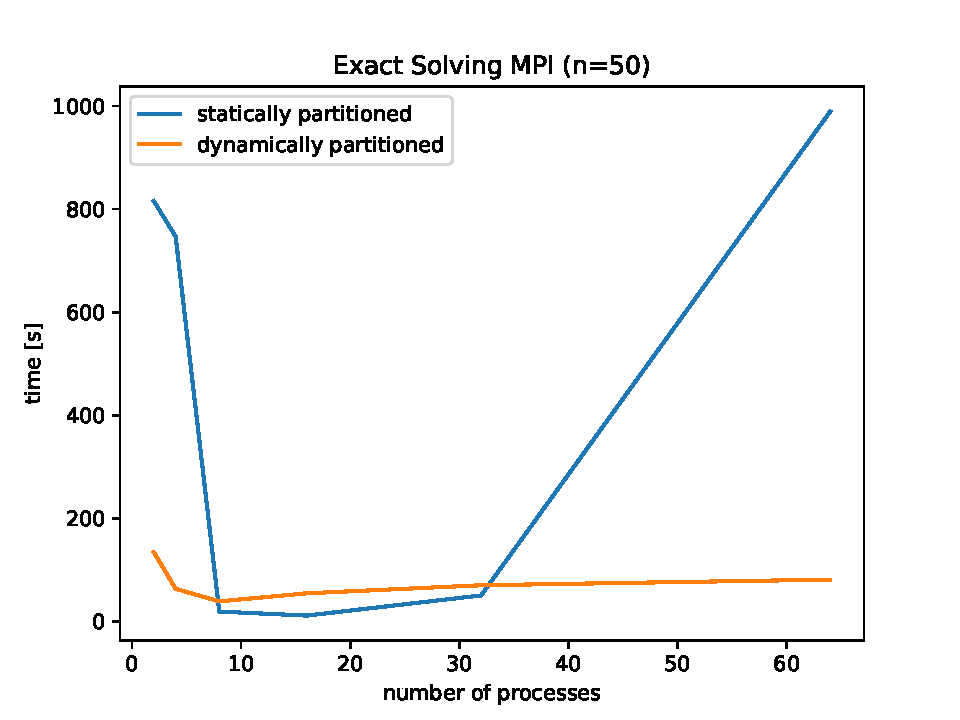
\includegraphics[width=0.8\textwidth]{./assets/exact-mpi.pdf}
  \caption{The comparison of the statically and dynamically allocated algorithm for different numbers of workers.}
\end{figure}

One can see that, averaged over all worker sizes, the dynamically partitioned algorithm performed better. This shows that, although more bits are sent, the more efficient allocation is worth the communication overhead. Furthermore, it is expected that the dynamically distributed algorithm performs comparatively better with more vertices, as more vertices increase the likelihood of an unfair static partitioning.

The optimal performance was recorded with the statically partitioned algorithm with 16 workers. Beyond 16 workers, the single coordinator becomes overwhelmed, resulting in longer waiting times for each worker to report their newly solved prefix.

Overall, it can be concluded that for smaller problems, the statically partitioned \ac{MPI} algorithm should be used, while for large graphs and more workers, the dynamically partitioned algorithm is preferred.

\subsubsection{MPI Analysis}

The \ac{MPI} analysis will be split into the statically partitioned and dynamically partitioned algorithm:

\paragraph{Statically partitioned}

Let $m$ be the number of workers, $n$ be the number of vertices in the graph, and $k$ the length of the prefix. Thus, including prefixes that do not form a proper subtour, we have 
\[
    n \cdot (n-1) \cdot (n-2) \cdot \dots \cdot (n-k) = \prod_{i=n-k}^n i
\]
prefixes. No communication is required for the prefix division. After each prefix, the worker sends $128$ bits\footnote{Assuming normal memory alignment.} to the coordinator and receives the global maximum back. Thus, excluding \ac{MPI} overhead, a total of $256 \cdot \prod_{i=n-k}^n i$ bits of data are sent in the actual computation. In the wrap-up, two broadcasts to $m-1$ nodes are done. But since those do not scale with $n$, they can be ignored in the overall complexity.

\paragraph{Dynamically partitioned}
Let $m$ be the number of workers and $n$ be the number of vertices. The prefix length is fixed to $3$. Thus, we have $n\cdot(n-1)\cdot(n-2) := n_{p}$ prefixes.

Each prefix gets assigned to a worker once, together with the current lowest minimum, resulting in $3\cdot64+64=256$ bits of data per message. For each prefix message to be sent, they have to be requested first. A request implicitly sends its rank and the current minimal path, thus $2\cdot64=128$ bits. Therefore, for the actual computation, a total of $n_p \cdot (128+256)$ bits are sent. Like with the statically partitioned solver, the wrap-up cost is independent of the graph size, and can therefore be ignored asymptotically.

\subsection{Nearest Neighbour benchmarks}

\subsubsection{Problem Size Scaling}
To compare the single-node sequential algorithm to the multithreaded version, starting at $n=100$, the graph size was increased in steps of $100$ up to $3000$. The results are as follows:

\begin{figure}[H]
  \centering
  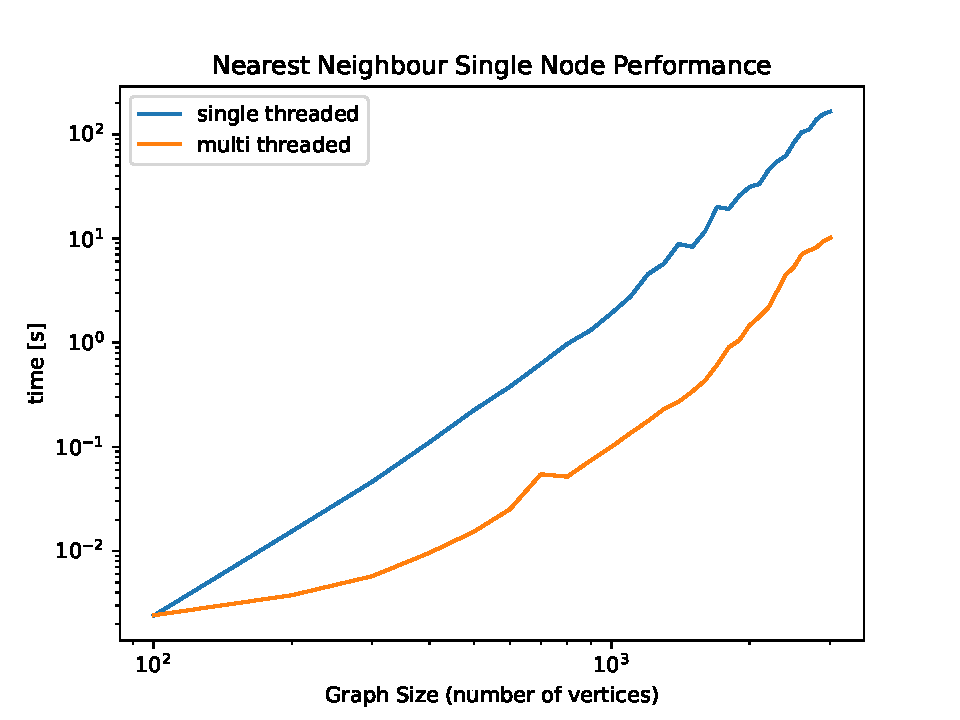
\includegraphics[width=0.8\textwidth]{./assets/nn-stmt.pdf}
  \caption{Problem Size scaling of the Nearest Neighbour algorithm}
\end{figure}

As one can see, in the beginning, the multithreading overhead keeps the problems performing more equally. Furthermore, while the multithreading is properly used, both algorithms keep the same asymptotic complexity. Overall, the nearest neighbour algorithm greatly benefits from multithreading. This was expected, as no inter-thread communication is required for computing the 1-nearest-neighbours. Furthermore, the minimum reduction at the end is single threaded in both versions, resulting in no overhead in the wrap-up.

\subsubsection{Strong Scaling}

For the \ac{MPI} analysis, a strong scaling benchmark was used, with a fixed graph size of $n=3000$. 

\begin{figure}[H]
  \centering
  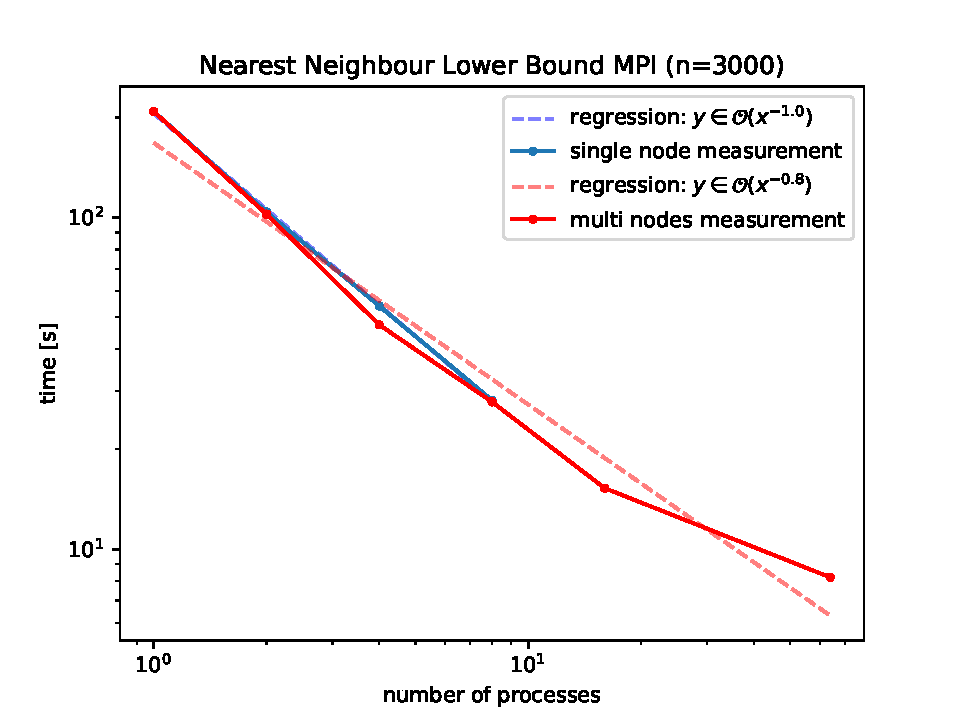
\includegraphics[width=0.8\textwidth]{./assets/NN-mpi.pdf}
  \caption{Strong scaling of the Nearest Neighbour algorithm}
\end{figure}

As one can see, the algorithm scales well with the amount of nodes. Analogously to the multithreading version, this was expected, as no inter-node communication is required for computing the single 1-nearest-neighbours. Furthermore, since the work partitioning is done locally on each node, no communication is needed for that either. Thus, with only two collective communications at all, \ac{MPI} provides very little overhead.

\subsubsection{MPI Analysis}
Let $m$ be the number of workers and $n$ be the number of vertices.

Since the actual computation does not require any communication, only the wrap-up sends any data at all, by first \texttt{ALL\_REDUCE} the best cost. After that, the best worker broadcasts the whole path. As the implementation of reductions is \ac{MPI}-dependent, it can only be assumed that an \texttt{ALL\_REDUCE} at most sends $m^2$ messages. Since it only sends the current best cost and its rank, it doesn't scale with the number of vertices and can therefore be ignored.

The broadcast at the end probably uses a tree structure internally, thus resulting in $n\cdot64+64$ bits being sent in $\log(m)$ time steps. Therefore, the communication scales linearly in the number of graph vertices.

\subsection{Christofides benchmarks}
\label{sec:christofides_bench}

\subsubsection{Problem Size Scaling}

\begin{figure}[H]
  \centering
  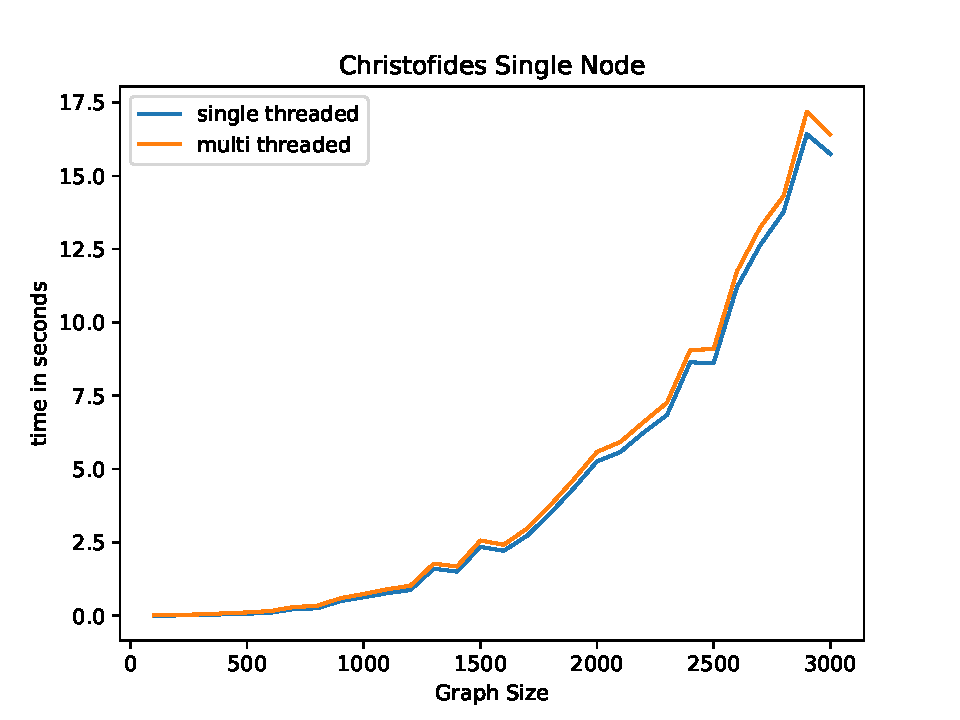
\includegraphics[width=\textwidth]{christofides-stmt.pdf}
  \caption{Problem Size scaling of the Christofides algorithm}
  \label{fig:weak_scaling_christofides}
\end{figure}
To compare the performance between the single-threaded implementation,
and the rayon-based implementation of the 1-tree lower bound,
a problem size scaling analysis is used.

In Figure \ref{fig:weak_scaling_christofides}, one can see that
the single-threaded implementation has roughly cubic
time complexity, w.r.t. the number of nodes in the input graph.

For the tested graph sizes, the multithreaded implementation
has no performance advantage, even the opposite is the case.
The rayon-based implementation has a worse runtime behaviour on all
tested graphs. Note, that the relative penalty diminishes
for larger graphs. For the reasoning, see the analogous problem in \ref{rayondoof}.

\subsubsection{Strong Scaling}

\begin{figure}[H]
  \centering
  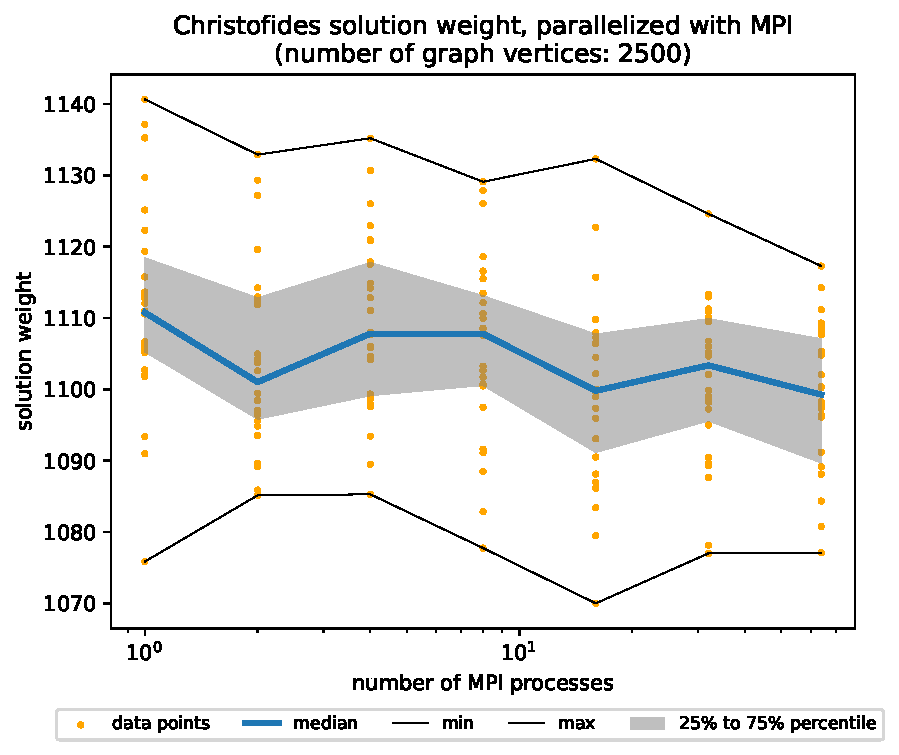
\includegraphics[width=\textwidth]{christofides-mpi.pdf}
  \caption{Strong scaling of the Christofides algorithm}
  \label{fig:strong_scaling_christofides}
\end{figure}

To assess the performance of the \ac{MPI}-based implementation of the Christofides algorithm,
a strong scaling analysis has been done, see Figure \ref{fig:strong_scaling_christofides}.

Note, that the \ac{MPI} implementation of the Christofides algorithm does not
use the parallelism to compute the result quicker, but rather
it uses the parallelism to compute a more precise result.
Hence, the format of the analysis differs from all the other ones.

Especially noticeable is, that the upper outliers get significantly smaller when 
using more processes, whereas the outliers to the bottom do not experience any more improvement.
This may be caused by worse initial solution guesses having greater potential for optimization,
and with more parallelism it is more likely to find a path for optimization.
In contrast, good initial guesses have less potential for optimization,
whereby added parallelism cannot help in that case.


\subsubsection{MPI Analysis}
For the algorithmic description look at 
the parallelization paragraph in section
\ref{paragraph:christofides_mpi}.

Let $p \geq 2$ be the number of \ac{MPI} processes.
Let $G = (V,E)$ be the input graph.
Then, during the execution of the \ac{MPI} variant of the Christofides algorithm,
$p-1$ tagged messages containing an \texttt{f64} value will be sent,
as well as $p-1$ tagged messages containing a vector of $|V| $ many \texttt{usize} values.
All of these messages will be received by the root process.
This will take the root process $\mathcal{O}(p \cdot |V|)$ time,
excluding time spent on synchronization, etc.

\subsection{1-tree Lower Bound}
\label{sec:1_tree_bench}

\subsubsection{Problem Size Scaling}

\begin{figure}[H]
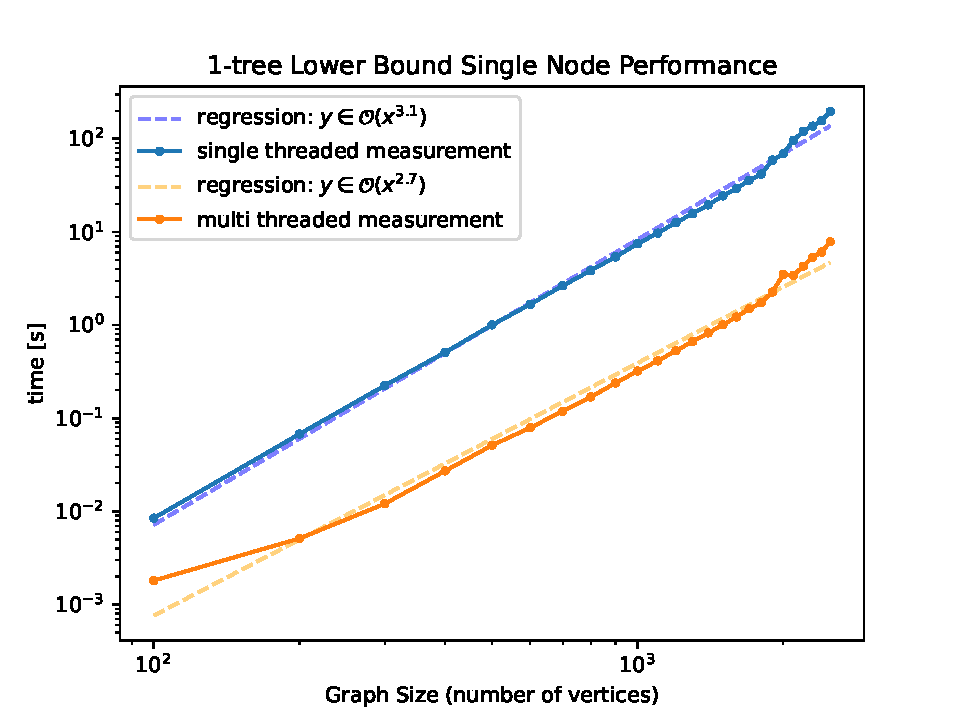
\includegraphics[width=\textwidth]{1-tree-stmt.pdf}
\caption{problem size scaling of the 1-tree lower bound}
\label{fig:weak_scaling_1_tree}
\end{figure}

To compare the performance between the single-threaded implementation,
and the rayon-based implementation of the 1-tree lower bound,
a problem size scaling analysis comes in handy.

As seen in Fig. \ref{fig:weak_scaling_1_tree},
both variants have roughly cubic time complexity,
with the multi-threaded variant being faster by a
constant factor.
This is an expected result, as the 1-tree lower bound of a graph $G = (V,E)$ essentially
involves computing $|V|$ many \ac{MST}s over $|V|-1$ vertices.
As can be seen in section \ref{sec:mst_bench}, for this implementation, the sequential computation of an \ac{MST}
has quadratic complexity, thus the cubic complexity of the 1-tree lower bound
follows easily.
The parallel implementation having a similar complexity, but being faster by a constant factor is also to be
expected since a constant number of \ac{MST} computations is done in parallel,
and other than that, nothing else is different from the sequential implementation.

\subsubsection{Strong Scaling}

\begin{figure}[H]
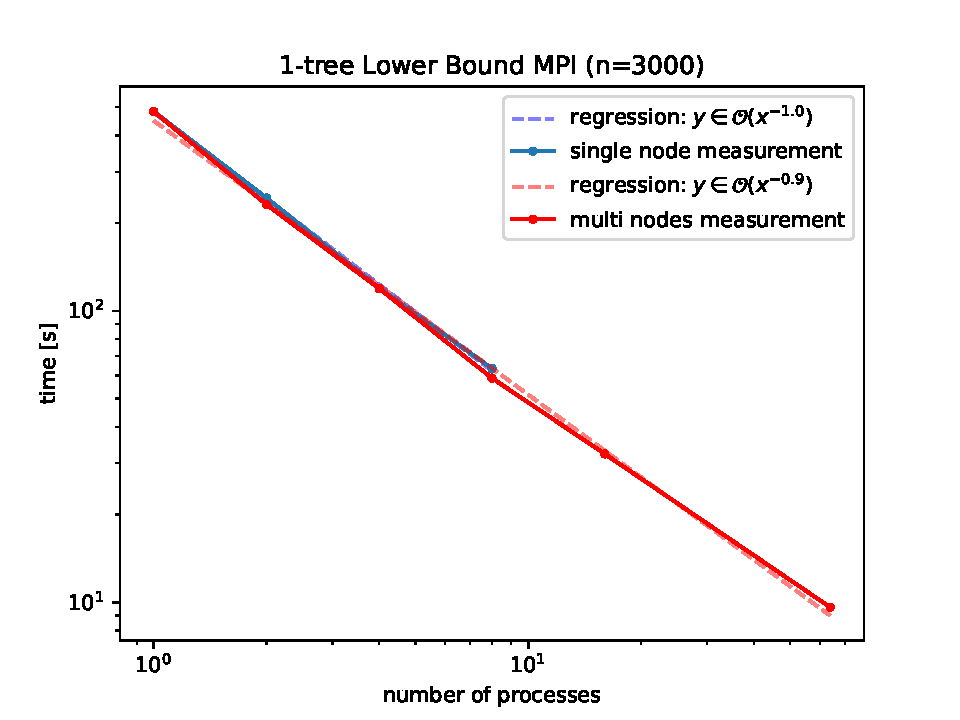
\includegraphics[width=\textwidth]{1-tree-mpi.pdf}
\caption{Strong scaling of the 1-tree lower bound}
\label{fig:strong_scaling_1_tree}
\end{figure}


To analyze, how the \ac{MPI} implementation
of the 1-tree lower bound
performs, a strong scaling analysis is applied.

As seen in Fig. \ref{fig:strong_scaling_1_tree},
the MPI implementation's performance is roughly
inversely proportional to the number of \ac{MPI} processes,
both when executed on only one host machine,
and when executed on multiple machines in a cluster.
This indicates, that the overhead of the \ac{MPI} runtime is negligible.


\subsubsection{MPI Analysis}

For the algorithmic description look at section \ref{sec:1-tree}.

Let $p \geq 2$ be the number of \ac{MPI} processes.
Let $G = (V,E)$ be the input graph.
During the execution of the \ac{MPI} variant of the 1-tree lower bound,
there is one \ac{MPI} communication happening:
After all processes have computed a lower bound, the maximum over all
local lower bounds is collected at the root process using an \ac{MPI} reduce operation.
This operation theoretically only needs $\mathcal{O}(\log p)$ time, and $\mathcal{O}(p)$ many
messages, by using a tree-like communication structure.
Practically, the performance of \ac{MPI} reduction operations is dependent on the concrete \ac{MPI} implementation
\cite[section 5.9]{message_passing_interface_forum_mpi_2015},
but the fact that the operation has been the subject of research for many years 
\cite{malyshkin_hierarchical_2015} suggests, that the established
\ac{MPI} implementations optimize the reductions.

Note, that the cost of the \ac{MPI} operations is independent of the graph size,
it only depends on the number of available processes.

\subsection{MST lower bound}
\label{sec:mst_bench}

\begin{figure}[H]
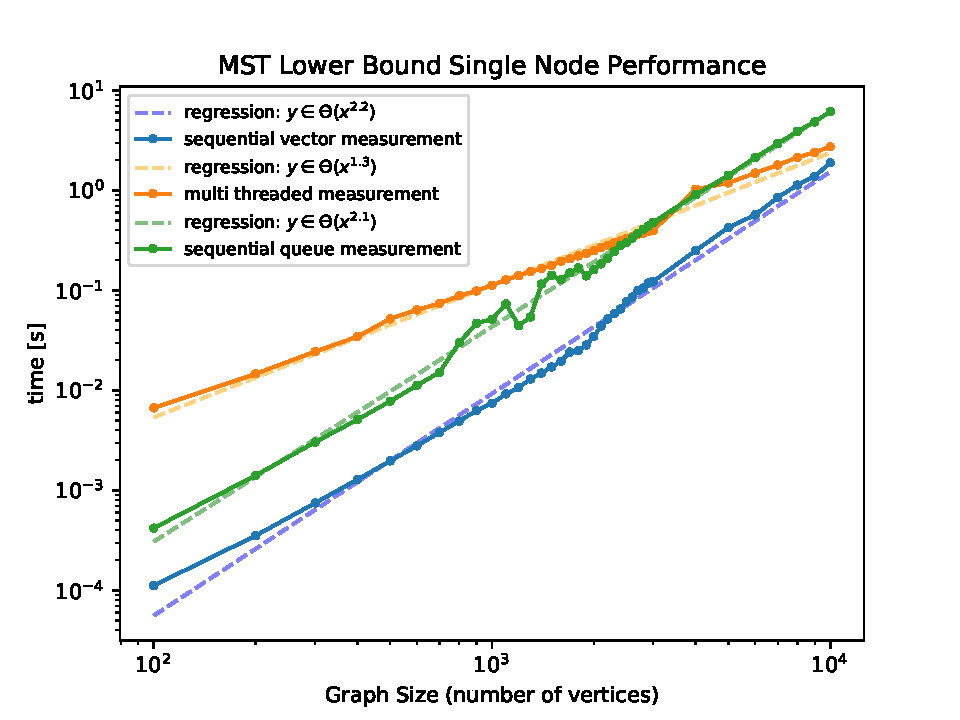
\includegraphics[width=\textwidth]{MST-all.pdf}
\caption{problem size scaling of the MST lower bound}
\label{fig:weak_scaling_mst}
\end{figure}

The \ac{MST} calculation has no \ac{MPI} implementation,
so only a problem size scaling analysis is performed.


There are three different implementations of Prim's algorithm provided:
a sequential, and a multi-threaded variant using linear search on vectors (see also \ref{sec:mst}),
and a sequential variant using a
priority queue\footnote{The priority queue is provided by the \texttt{priority-queue} crate \cite{garro95_priorityqueue_2023}}.
As the reader can see in Figure \ref{fig:weak_scaling_mst},
the sequential vector-based algorithm performs best,
for all tested inputs, and has roughly quadratic runtime behaviour,
w.r.t. the number of nodes in the input graph.

Interestingly, the priority queue-based implementation is neither quicker
nor does it show slower growth, than the sequential vector-based implementation.
This may be explained with
a sub-par third-party implementation of the priority queue data structure,
or with insufficient input size. Note, that the largest tested graph (10,000 vertices)
takes 4.6 GiB of disk space in TSPLIB-XML format.

The multithreaded variant does not outperform the sequential vector-based implementation,
though for graphs a little larger than 10,000 vertices it probably would have.
It did however scale nearly linearly w.r.t. number of vertices,
even though asymptotically, its runtime behaviour is equivalent to the sequential vector-based implementation.
This may be, because the smaller the graphs are,
the more the overhead of multithreading dominates over
the benefit of it.
